%* 
%* ------------------------------------------------------------------
%* TTReference.tex - Time Table (V2) Reference
%* Created by Robert Heller on Thu Apr 26 12:33:54 2007
%* ------------------------------------------------------------------
%* Modification History: $Log$
%* Modification History: Revision 1.1  2007/05/06 12:49:40  heller
%* Modification History: Lock down  for 2.1.8 release candidate 1
%* Modification History:
%* Modification History: Revision 1.1  2002/07/28 14:03:50  heller
%* Modification History: Add it copyright notice headers
%* Modification History:
%* ------------------------------------------------------------------
%* Contents:
%* ------------------------------------------------------------------
%*  
%*     Model RR System, Version 2
%*     Copyright (C) 1994,1995,2002-2005  Robert Heller D/B/A Deepwoods Software
%* 			51 Locke Hill Road
%* 			Wendell, MA 01379-9728
%* 
%*     This program is free software; you can redistribute it and/or modify
%*     it under the terms of the GNU General Public License as published by
%*     the Free Software Foundation; either version 2 of the License, or
%*     (at your option) any later version.
%* 
%*     This program is distributed in the hope that it will be useful,
%*     but WITHOUT ANY WARRANTY; without even the implied warranty of
%*     MERCHANTABILITY or FITNESS FOR A PARTICULAR PURPOSE.  See the
%*     GNU General Public License for more details.
%* 
%*     You should have received a copy of the GNU General Public License
%*     along with this program; if not, write to the Free Software
%*     Foundation, Inc., 675 Mass Ave, Cambridge, MA 02139, USA.
%* 
%*  
%* 

\chapter{Time Table (V2) Reference}
\label{chpt:tt:Reference}
\typeout{$Id$}

The Time Table (V2) program is a hybrid program, consisting of a Tcl/Tk
GUI on top of a C++ class library.  The GUI provides the user interface
to the algorithms and data structures contained in the C++ class
library.  This program was inspired by chapter 8 of the book {\it How
to Operate Your Model Railroad}\cite{Chubb77} by Bruce A. Chubb.  I
strongly recommend reading this chapter fully before using this
program.  This program implements the methods described in this
chapter, in an automated fashion.

\section{Command Line Usage}

\begin{figure}[hbpt] 
\begin{centering} 
{\footnotesize
\begin{verbatim} 
TimeTable oldtimetablefile 
TimeTable -totaltime time -timeincrement time nameoftimetable 
\end{verbatim} 
}
\caption{Command Line Format for the TimeTable command} 
\label{fig:tt:cliusage} 
\end{centering} 
\end{figure}
There are two formats for the TimeTable program's command line.  The
command line can either have a single file name, the name of an
existing time table file or it can have two options (\texttt{-totaltime}
and \texttt{-timeincrement}) and the name of a new time table.  The first
form loads an existing time table (see
Section~\ref{sect:tt:loadexistingtimetable} and the second form creates
a new time table (see Section~\ref{sect:tt:createnewtimetable}.  These
two command line formats are shown in Figure~\ref{fig:tt:cliusage}. 

\section{Layout of the Main GUI}

\begin{figure}[hbpt]
\begin{centering}
\includegraphics[width=5in]{TTMainGUIBlank.png}
\caption{The main GUI screen of the Time Table (V2) Program}
\label{fig:tt:MainGUIBlank}
\end{centering}
\end{figure}
\begin{figure}[hbpt]
\begin{centering}
\includegraphics[width=5in]{TTMainGUIToolBar.png}
\caption{The Toolbar of the Time Table (V2) Program}
\label{fig:tt:MainGUIToolBar}
\end{centering}
\end{figure}
\begin{figure}[hbpt]
\begin{centering}
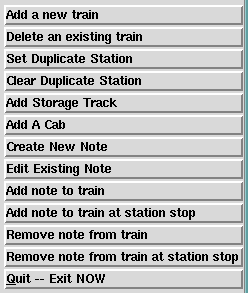
\includegraphics{TTMainGUIButtonMenu.png}
\caption{The Button Menu of the Time Table (V2) Program}
\label{fig:tt:MainGUIButtonMenu}
\end{centering}
\end{figure}
The main GUI window\index{Time Table!main GUI}, show in
Figure~\ref{fig:tt:MainGUIBlank}, contains a menu bar, a toolbar
(Figure~\ref{fig:tt:MainGUIToolBar}), a time table chart, and a button
menu (Figure~\ref{fig:tt:MainGUIButtonMenu}).

\section{Creating a New Time Table}
\label{sect:tt:createnewtimetable}

\begin{figure}[hbpt]
\begin{centering}
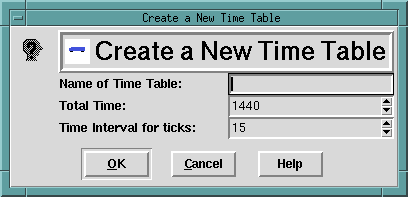
\includegraphics{TTCreateNewTT.png}
\caption{Create A New Time Table dialog}
\label{fig:tt:GetNewTimeTableDialog}
\end{centering}
\end{figure}
Creating a new time table can be done from the command line by
specifying a total time (in minutes) value with the \texttt{-totaltime}
option and a time increment value (in minutes) value with the
\texttt{-timeincrement} option and a name for the new time table (as
shown in the second line of Figure~\ref{fig:tt:cliusage}).  A new time
table can also be created with the \texttt{New} menu item of the
\texttt{File} menu or the

\includegraphics{TTNewTool.png} toolbar button. These later two methods
use the ``Create a New Time Table'' dialog, shown in
Figure~\ref{fig:tt:GetNewTimeTableDialog} to get the total time, time
increment, and the name of the new time table.  If there is a time
table file already loaded, a confirmation dialog will be displayed.

\subsection{Creating the station stops for a new time table}
\label{sect:tt:CreateAllStationsDialog}

\begin{figure}[hbpt]
\begin{centering}
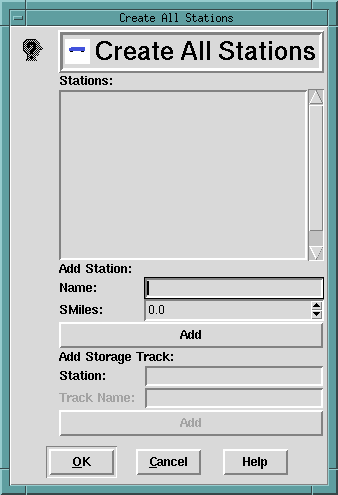
\includegraphics{TTCreateAllStations.png}
\caption{Create All Stations Dialog}
\label{fig:tt:CreateAllStationsDialog}
\end{centering}
\end{figure}
Stations for a time table must all be created when the time table is
created.  Stations cannot be added or removed later.  When a new time
table is created the ``Create All Stations Dialog'',  shown in
Figure~\ref{fig:tt:CreateAllStationsDialog} is displayed to create all
of the station stops.

\subsection{Creating an initial set of ``cabs''}

\begin{figure}[hbpt]
\begin{centering}
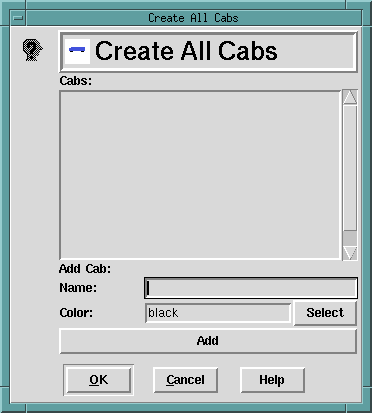
\includegraphics{TTCreateAllCabs.png}
\caption{Create All Cabs Dialog}
\label{fig:tt:CreateAllCabsDialog}
\end{centering}
\end{figure}
Once the stations have been created, an initial set of ``cabs'' can be
created.  Commonly, cabs are only used on block switch DC layouts, but
the cabs can be used as with a  DCC layout as a way to associate trains
with different operating ``crews'' (operators) or just to identify
different classes of trains by color, etc.  The ``Create All Cabs''
dialog, shown in Figure~\ref{fig:tt:CreateAllCabsDialog}, is used to
bulk create an initial set of cabs.

\begin{figure}[hbpt]
\begin{centering}   
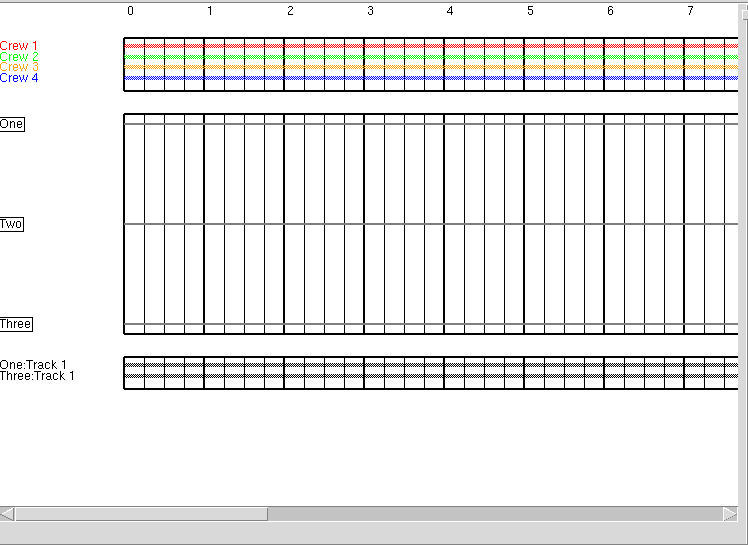
\includegraphics[width=5in]{TTChart3station.png}
\caption{Simple chart with three stations, four cabs, and two storage
tracks}
\label{fig:tt:Chart3station}
\end{centering}
\end{figure}   
A simple chart with three stations, four cabs (labeled ``Crew 1''
through ``Crew 4''), and two storage tracks is shown in
Figure~\ref{fig:tt:Chart3station}. 

\section{Loading an Exiting Time Table File}
\label{sect:tt:loadexistingtimetable}

An existing time table file can be loaded from the command line (as
shown in the first line of Figure~\ref{fig:tt:cliusage}),  with the
\texttt{Open...} menu item of the \texttt{File} menu or the

\includegraphics{TTOpenTool.png} toolbar button. If there is a time
table file already loaded, a confirmation dialog will be displayed.

\section{Saving a Time Table File}

The currently loaded time table can be saved with either the
\texttt{Save} (or \texttt{Save As...}) menu item of the \texttt{File} menu or
the \includegraphics{TTSaveTool.png} toolbar button. 

\section{Adding Trains}

Trains are added using the either the \texttt{Add Train} menu item of the
\texttt{Trains} menu, clicking on the add train
(
\includegraphics{TTaddtrain.png}) toolbar button or the \texttt{Add a
new train} button. All of these display the ``Create New Train
Dialog'', described in Section~\ref{sect:tt:CreateNewTrainDialog}.

\subsection{Create New Train Dialog}
\label{sect:tt:CreateNewTrainDialog}

\begin{figure}[hbpt]
\begin{centering}   
\includegraphics{TTCreateNewTrain1.png}
\caption{Creating a new train dialog, basic information}
\label{fig:tt:CreateNewTrain1}
\end{centering}
\end{figure}
The ``Create New Train Dialog'' first collects some basic information
about the new train, as shown in Figure~\ref{fig:tt:CreateNewTrain1}.
The basic train information consists of the train's common name, its
number (or symbol), its class number, its average speed, its scheduled
departure time, and the two stations it travels between.

The train's number (or symbol) needs to be a unique identification of
the train.  The common name need not be unique.  The class is a whole
number, with smaller numbers generally being the ``higher'' class. The
class is used to indicate a train's priority and is also used to group
similar trains together.  The speed is the (scale) speed the train will
be traveling between stops.  The scheduled departure time is the time
the train is scheduled to leave its origin station.  The origin and
termination stations are the station end points the train travels between.

\begin{figure}[hbpt]
\begin{centering}   
\includegraphics[width=5in]{TTCreateNewTrain2.png}
\caption{Creating a new train dialog, scheduling information}
\label{fig:tt:CreateNewTrain2}
\end{centering}
\end{figure}
The \texttt{Schedule} button selects the scheduling page of the ``Create a
New Train Dialog'', as shown in Figure~\ref{fig:tt:CreateNewTrain2}.  On
this page, the cab can be selected and layover periods at intermediate
stations can be set.  The \texttt{Update} buttons propagate the cab
settings and adjust the times to allow for the layovers.

\begin{figure}[hbpt]
\begin{centering}   
\includegraphics{TTCreateNewTrain3.png}
\caption{Creating a new train dialog, storage track selection}
\label{fig:tt:CreateNewTrain3}
\end{centering}
\end{figure}
The \texttt{Storage} button selects the storage track allocation page of
the ``Create a New Train Dialog'', as shown in
Figure~\ref{fig:tt:CreateNewTrain3}.  This page lists those stations
that have storage tracks available.  It only makes sense to select
storage tracks for intermediate stops if there is a layover or for
originating or terminating stops.

\section{Deleting Trains}
\label{sect:tt:DeletingTrains}

Trains are deleted using the \texttt{Delete Train} menu item of the
\texttt{Trains} menu, clicking on the delete train
(
\includegraphics{TTdeletetrain.png}) toolbar button or the
\texttt{Delete an Existing train} button. All of these display the
``Select One Train Dialog'', described in
Section~\ref{sect:tt:SelectOneTrainDialog}. A delete confirmation
dialog will also be displayed.

\section{Linking and Unlinking Duplicate Stations}

Duplicate stations occur mostly with ``out and back'' type layouts
where the opposite ends of the line are modeled with the same trackage
(usually a yard).  Duplicate stations also occur with reverse loops. In
all cases, these are stations which are logically different, but which
use the same tracks. There is an example in Figure~8-4 on page 86 of
\cite{Chubb77}. It is necessary to keep track of this trackage in the
schedule.  The duplicate station linking handles this. Duplicate
stations need to be setup before trains have been added.

The \texttt{Set Duplicate Station} and 
\texttt{Clear Duplicate Station} menu items of the \texttt{Stations} menu, the
\includegraphics{TTsetdupstation.png} and

\includegraphics{TTcleardupstation.png} toolbar buttons, and the
\texttt{Set Duplicate Station} and \texttt{Clear Duplicate Station} buttons
set and clear duplicate stations.

\section{Adding Station Storage Tracks}

Storage tracks are sidings where whole trains can be stored, either
during a long layover or between trips. The  \texttt{Add Storage Track}
menu item of the \texttt{Stations} menu, the

\includegraphics{TTaddstorage.png} toolbar button, or the  \texttt{Add
Storage Track} button are used to add a storage track to a station.

\section{Adding Cabs}

Generally ``Cabs'' refer to the separate throttle controls on a block
switched DC layout.  They are generally non-existent with a DCC layout,
but virtual cabs might be used as a way of assigning crews (operators)
to a train or to a segment of a train's run.  Cabs are added with the
\texttt{Add A Cab} menu item of the \texttt{Cabs} menu, the

\includegraphics{TTaddcab.png} toolbar button or the \texttt{Add A Cab}
button.

\section{Handling Notes}

Notes are brief memos about the operating rules in effect.  There is a
single pool of notes.  Notes from this pool can be associated either
with a whole train or with a train at a station stop.  The notes can
specify schedule exceptions (eg ``Daily except Saturdays, Sundays, and
Holidays''), or operating rules relating to meets.

\subsection{Creating New Notes and Editing Existing Notes}

\begin{figure}[hbpt]
\begin{centering}   
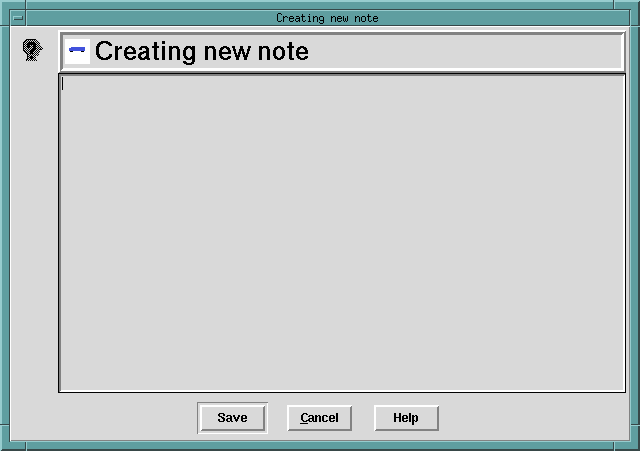
\includegraphics[width=5in]{TTEditNote.png}
\caption{Note editor dialog}
\label{fig:tt:EditNote}
\end{centering}
\end{figure}
Notes are created and edited the \texttt{Create New Note} and
\texttt{Edit Existing Note} menu items of the \texttt{Notes} menu, the

\includegraphics{TTcreatenote.png} and \includegraphics{TTeditnote.png}
toolbar buttons, or the \texttt{Create New Note} and 
\texttt{Edit Existing Note} buttons.  The the ``Note editor dialog'', shown in
Figure~\ref{fig:tt:EditNote} is used to create or edit the note.  Notes are
numbered consecutively starting with 1.

\subsection{Adding and Removing a Notes To Trains}

\begin{figure}[hbpt]
\begin{centering}
\includegraphics{TTAddNote.png}
\caption{Add (or Remove) Note dialog}
\label{fig:tt:AddNote}
\end{centering}
\end{figure}
Notes are added to trains or removed from trains with \texttt{Notes} menu
items \texttt{Add note to train}, \texttt{Add note to train at station stop},
\texttt{Remove note from train}, and 
\texttt{Remove note from train at station stop}; the
\includegraphics{TTaddnotetotrain.png},
\includegraphics{TTaddnotetotrainatstation.png},
\includegraphics{TTremovenotefromtrain.png}, and

\includegraphics{TTremovenotefromtrainatstation.png}; or the  
\texttt{Add note to train}, \texttt{Add note to train at station stop}, 
\texttt{Remove note from train}, and 
\texttt{Remove note from train at station stop} buttons.  All of these
display the ``Add (or Remove) Note dialog'', shown in
Figure~\ref{fig:tt:AddNote}.

\section{Printing a Time Table}

``Printing'' a time table actually means creating a \LaTeX{} file and
then processing that \LaTeX{} file through a \LaTeX{} processing program
(typically \texttt{pdflatex}).  \LaTeX{} provides the means to produce a
professionally formatted document and has the means to provide things
like table of contents and the creation of a final document in a
selection of different final formats, including PDF (via
\texttt{pdflatex}), PostScript (via \texttt{latex} and \texttt{dvips})
or HTML (via the \texttt{htlatex} script from \textit{tex4ht} package).

Much of the formatting is customizable through the insertion of \LaTeX{}
code fragments as well as through various parameter settings.  It is
also possible to edit the \LaTeX{} style file that comes with the Time
Table program (\texttt{TimeTable.sty}) to tweak some of the fine details
of the formatting as well\footnote{Some knowledge of how \LaTeX{} works
is recommended when messing with the style file.}.

The \texttt{Print} menu item of the \texttt{File} menu or the
\includegraphics{TTprintTool.png} toolbar button initiate the print
process by displaying the ``Print Timetable'' dialog, described in
Section~\ref{sect:tt:PrintTimetableDialog}.


\subsection{Print Timetable Dialog}
\label{sect:tt:PrintTimetableDialog}

\begin{figure}[hbpt]
\begin{centering}
\includegraphics[width=5in]{TTPrintTimetableDialog.png}
\caption{Print Timetable dialog}  
\label{fig:tt:PrintTimetableDialog}
\end{centering}
\end{figure}
The ``Print Timetable'' dialog, shown in
Figure~\ref{fig:tt:PrintTimetableDialog}, collects the basic
information needed to generate and process a \LaTeX{} source file from
the time table data structure.  This information consists of the name of
the name of the \LaTeX{} source file to create, the \LaTeX{} processing
program (\texttt{pdflatex} by default), whether to run the \LaTeX{}
processing three times (to get the table of contents right), the name of
any post processing command (such as \texttt{dvips} if using plain
\texttt{latex}).  Most of the time, this is enough for a standard, basic
time table.  The \texttt{Configure} button can be used to configure a
selection of options using a ``Print Configuration'' dialog, described
in Section~\ref{sect:tt:PrintConfigurationDialog}.

Once the settings and configuration have been set, the \texttt{Print}
initiates the process.  First a \LaTeX{} source file is generated, then
the \LaTeX{} processing program is run once or three times.  The output
from these runs are displayed in a process log window (\LaTeX{} outputs
a fair amount of diagnostic output, most of which can be ignored).  If
you are using the default processor (\texttt{pdflatex}), you should now
have a PDF file which can be viewed or printed with the PDF viewer of
your choice.

\subsection{Print Configuration Dialog}
\label{sect:tt:PrintConfigurationDialog}

\begin{figure}[hbpt]
\begin{centering}
\includegraphics[width=5in]{TTPrintConfigurationDialog1.png}
\caption{Print Configuration dialog, General settings}
\label{fig:tt:PrintConfigurationDialog1}
\end{centering}
\end{figure}
\begin{figure}[hbpt]
\begin{centering}
\includegraphics[width=5in]{TTPrintConfigurationDialog2.png}
\caption{Print Configuration dialog, Multi settings}
\label{fig:tt:PrintConfigurationDialog2}
\end{centering}
\end{figure}
\begin{figure}[hbpt]
\begin{centering}
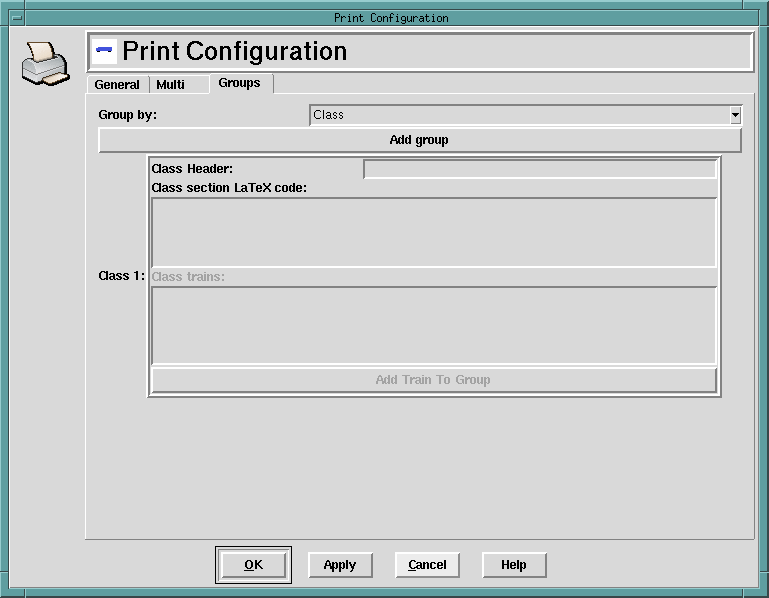
\includegraphics[width=5in]{TTPrintConfigurationDialog3.png}
\caption{Print Configuration dialog, Groups settings}
\label{fig:tt:PrintConfigurationDialog3}
\end{centering}
\end{figure}
The Print Configuration Dialog, shown in
Figures~\ref{fig:tt:PrintConfigurationDialog1};
\ref{fig:tt:PrintConfigurationDialog2}; and
\ref{fig:tt:PrintConfigurationDialog3}, provide for the setting of many
print configuration options. The general settings
(Figure~\ref{fig:tt:PrintConfigurationDialog1}), provide for setting the
title, subtitle, the date, whether to have \LaTeX{} format for double
sided printing, setting the time format, setting the logical direction
of trains, column widths, and including additional commands in the
\LaTeX{} preamble (usually including additional style
packages\footnote{The style pages supertabular and graphicx are already
included.} and style settings). The multi-table settings
(Figure~\ref{fig:tt:PrintConfigurationDialog2}), provide for settings
relating to time tables using multiple tables.  These settings include
whether to create a table of contents, whether to use multiple tables at
all, \LaTeX{} code to precede the table of contents, \LaTeX{} code to
precede notes section, the header to use if a single ``All Trains''
table is generated, and \LaTeX{} code to precede this single ``All
Trains'' table.  The groups settings
(Figure~\ref{fig:tt:PrintConfigurationDialog3}), provide for settings
for each group.  This includes whether to group by class or to manually
group trains and provides for setting the class or group heading and for
\LaTeX{} code to precede the group table, and if grouping manually,
selecting the trains in the group.

\section{Exiting From the Program}

The \texttt{Exit} (or \texttt{Close}) menu item of the \texttt{File}
menu, the 
\includegraphics{TTCloseTool.png} toolbar button, or the
\texttt{Quit -- Exit NOW} button exit the program.  A confirmation
dialog is displayed to get confirmation.

\section{Select One Train Dialog}
\label{sect:tt:SelectOneTrainDialog}

\begin{figure}[hbpt] 
\begin{centering}
\includegraphics{TTSelectOneTrain.png} 
\caption{Select One Train dialog} 
\label{fig:tt:SelectOneTrainDialog} 
\end{centering}
\end{figure} The ``Select One Train dialog'', shown in
Figure~\ref{fig:tt:SelectOneTrainDialog}, is used to select a train
either for deletion (Section~\ref{sect:tt:DeletingTrains}) or for
viewing (Section~\ref{sect:tt:ViewingTrains}).

\section{The View Menu}

The view menu contains menu items for viewing detailed information about
various things, including trains (Section~\ref{sect:tt:ViewingTrains},
stations (Section~\ref{sect:tt:ViewingStations}), and  notes
(Section~\ref{sect:tt:ViewingNotes}).

\subsection{Trains}
\label{sect:tt:ViewingTrains}

There are two menu items for viewing trains, \texttt{View One Train} and
\texttt{View All Trains}.  The \texttt{View One Train} uses the ``Select
One Train dialog'' (Section~\ref{sect:tt:SelectOneTrainDialog}) to
select a train to display detailed information about and the
\texttt{View All Trains} menu item displays a dialog listing all of the
trains, by number and name, with buttons to get more detailed information.

\subsection{Stations}
\label{sect:tt:ViewingStations}

There are two menu items for viewing stations, \texttt{View One
Station} and \texttt{View All Stations}.  The \texttt{View One Station}
uses the ``Select One Station dialog'' to select a station to display
detailed information about and the \texttt{View All Stations} menu item
displays a dialog listing all of the stations, by name and scale mile, with
buttons to get more detailed information.

\subsection{Notes}
\label{sect:tt:ViewingNotes}

There are two menu items for viewing notes, \texttt{View One Note} and
\texttt{View All Notes}.  The \texttt{View One Note} uses the ``Select
One Note dialog'' to select a note to display detailed information
about and the \texttt{View All Notes} menu item displays a dialog
listing all of the notes, by number and beginning text, with buttons to
get more detailed information.

\section{System Configuration}

The Time Table program has a small number of global
configuration options.  These are stored in a file named
\texttt{.timeTable} (\texttt{TimeTable.rc} under MS-Windows) in the
current user's HOME directory.  These configuration options are:
\begin{description}
\item [Path to pdflatex] The pathname to the \texttt{pdflatex}
executable.
\item [Label Width in Chart] The width in pixels of cab, station, and
storage track labels in the time table chart.
\item [Height of main window] The initial height of the main window.
\item [Width of main window] The initial width of the main window.
\end{description}

The system configuration file is read at program startup.  If the
configuration does not exist, a default one is created the first time
the program is run.

The \texttt{Options} menu manages the system configuration, with menu
items to edit the system configuration, save it and reload it.

\section{Add Cab Dialog}
\section{Add Remove Note Dialog}
\section{Create All Cabs Dialog}
\section{Create All Stations Dialog}
\section{Create A New Time Table Dialog}
\section{Edit Note Dialog}
\section{Edit System Configuration}
\section{Edit Train Dialog}
\section{Print Configuration Dialog}
\section{Print Dialog}
\section{Select A Storage Track Name}
\section{Select One Note Dialog}
\section{Select One Station Dialog}
\section{Select One Train Dialog}
